\documentclass{article}
\usepackage{blindtext}
\usepackage{authblk}
\usepackage[utf8]{inputenc}
\usepackage{amsmath, amssymb}
\usepackage{amssymb}
\usepackage[overload]{empheq}
\usepackage[font=small,labelfont=bf]{caption}
\usepackage{subcaption}
 % Required for specifying captions to tables and figures

\newcommand{\for}{\text{for }}
 
\title{SPM project: Parallel Prefix}
\author{Gaspare Ferraro, 520549}
\affil{Master Degree in Computer Science - University of Pisa}
\affil[]{ferraro@gaspa.re}
\date{\today}
 
\begin{document}
 
\maketitle
 
%%%%%%%%%%%%%%%%%%%%%%%%%%%%%%%%%%%%%%%%%%%%%%%%%%%%%%%%%%%%%%%%%%%%%%%%%%%%%%%
\section{Introduction}

In this report we will analyze, theoretically and practically, the resolution of the problem of the (parallel) prefix sum:

\medskip

\textit{Given a vector $x = \langle x_{0}, x_{1}, \ldots, x_{n-1} \rangle$ and a binary operation $\oplus$ compute the vector $y = \langle x_{0}, x_{0} \oplus x_{1}, x_{0} \oplus x_{1} \oplus x_{2}, \ldots, x_{0} \oplus x_{1} \oplus \ldots \oplus x_{n-1} \rangle$.} % , i.e. each element of the output vector at position $i$ is the results of 

\medskip

In literature this operation is also called (inclusive) scan or partial sum.

For the analysis of the problem we have to make two assumptions:

\begin{itemize}
  \item The binary operation $\oplus$ is associative ($ a \oplus ( b \oplus c ) =  (a \oplus b) \oplus c  $) and commutative ($a \oplus b = b \oplus a$), this is an important assumption as we will see in the next chapters the order of the operations may not be preserved.
  \item The size of the input vector is a power of $2$, not a strong assumption, as all the algorithms we will present could be easily generalize to all the sizes, but it only helps to simplify some operations.
\end{itemize}

%%%%%%%%%%%%%%%%%%%%%%%%%%%%%%%%%%%%%%%%%%%%%%%%%%%%%%%%%%%%%%%%%%%%%%%%%%%%%%%
\section{Sequential algorithm}

The sequential algorithm simple compute each element of the vector $y$ as follow:

\begin{equation*}[]
    y_{i} =
    \begin{cases}
      x_{0}& \for i = 0 \\
      x_{i} \oplus y_{i-1},& \for 0 <  i < n
    \end{cases}
\end{equation*}

This algorithm is optimal in a sequential model as it has a running time of $\mathcal{O}(n)$, assuming that $\oplus$ is $\mathcal{O}(1)$, and performs $n-1$ calls to $\oplus$ operation.
 
%%%%%%%%%%%%%%%%%%%%%%%%%%%%%%%%%%%%%%%%%%%%%%%%%%%%%%%%%%%%%%%%%%%%%%%%%%%%%%%
\section{Parallel architecture design}

The problem of computing the prefix sum vector is a classical example of a problem that have an optimal solution in a sequential model but that can be optimized in a parallel model. 
The optimization is not in terms of total complexity or in the number of $\oplus$ operations performed (which are already optimals in the sequential algorithm) but in terms of completion time. When the number of available threads is more than one we can trade-off more total work for less completion time.
\medskip

We will now introduce two different algorithms that solve in an efficient way the prefix sum problem in a parallel model. 

\subsection{Block-based algorithm}

The idea behind the first parallel algorithm is to compute the prefix vector in three phases:

\begin{itemize}
  \item Partitionate the input vector in blocks and compute in parallel the prefix vector of each of them.
  \item In the second phase we put the final element of each block in a temporary vector and compute its prefix vector.
  \item Finally for each block $i$ (except for the first one) add in parallel the $(i-1)$th element of the temporary vector.
\end{itemize}

At the end of the three phases the final vector contains the correct prefix .

\begin{center}
\begin{minipage}{0.75\linewidth}
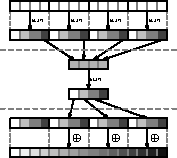
\includegraphics[width=\linewidth]{img/block}
\captionof{figure}{Block-based algorithm graphic representation} 
\end{minipage}
\end{center}

\subsection{Circuit-based algorithm}

Another kind of algorithms are the one based on a circuit-like representation, 

A generic prefix circuit $C$ is a collections of sets 

For example the serial algorithm seen before can be represented as a prefix circuit $S(n) = \{ G_{0}, G_{1}, \ldots, G_{n-1} \}$ where $G_{i} = \{ (i, i+1) \}$.

We present now the simple (but still efficient) prefix circuit $P(2^m)$:

\begin{equation*}
  
\end{equation*}

In the first phase (from $t = 1$ to $t = m$) we compute operations like

In the second phase (from $t = m+1$ to $t = 2m -1$) we compute the final value of 

\begin{figure}[h]
\centering
\begin{subfigure}{.5\textwidth}
  \centering
  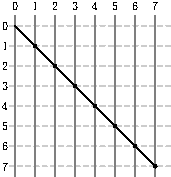
\includegraphics[width=.9\linewidth]{img/circuit-serial}
  \caption{Prefix circuit $S(8)$}
  \label{fig:sub1}
\end{subfigure}%
\begin{subfigure}{.5\textwidth}
  \centering
  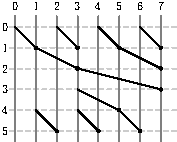
\includegraphics[width=.9\linewidth]{img/circuit-parallel}
  \caption{Prefix circuit $P(8)$}
  \label{fig:sub2}
\end{subfigure}
\caption{Examples of prefix circuits}
\label{fig:test}
\end{figure}

%%%%%%%%%%%%%%%%%%%%%%%%%%%%%%%%%%%%%%%%%%%%%%%%%%%%%%%%%%%%%%%%%%%%%%%%%%%%%%%
\section{Performance modeling}

 
\subsection{Block-based algorithm}


\subsection{Circuit-based algorithm}


%%%%%%%%%%%%%%%%%%%%%%%%%%%%%%%%%%%%%%%%%%%%%%%%%%%%%%%%%%%%%%%%%%%%%%%%%%%%%%%
\section{Implementations structure and details}

All the implementations are written in $C++17$, the source code is available as attachment with the report or on GitHub

 (https://github.com/GaspareG/ParallelPrefix).


\subsection{Sequential algorithm}

The sequential implementations 

\subsection{Block-based algorithm}

TODO

\subsection{Circuit-based algorithm}

TODO

%%%%%%%%%%%%%%%%%%%%%%%%%%%%%%%%%%%%%%%%%%%%%%%%%%%%%%%%%%%%%%%%%%%%%%%%%%%%%%%
\section{Experimental validation}


\subsection{experiments details}

\subsection{benchmark results}

%%%%%%%%%%%%%%%%%%%%%%%%%%%%%%%%%%%%%%%%%%%%%%%%%%%%%%%%%%%%%%%%%%%%%%%%%%%%%%%
\section{Conclusion}


%%%%%%%%%%%%%%%%%%%%%%%%%%%%%%%%%%%%%%%%%%%%%%%%%%%%%%%%%%%%%%%%%%%%%%%%%%%%%%%
\end{document}
